\documentclass[a4paper,10pt,twoside,openany]{book}

\usepackage[lang=hebrew]{maths}
\usepackage{hebrewdoc}
\usepackage{stylish}
\usepackage{lipsum}
\let\bs\blacksquare

\setlength{\parindent}{0pt}

%%%%%%%%%%%%
% Styling %
%%%%%%%%%%%%

\usepackage{enumitem}

%%%%%%%%%%%%%
% Counters  %
%%%%%%%%%%%%%

\setcounter{section}{1}     
            
%BIBLIOGRAPHY
\usepackage[
backend=biber,
style=alphabetic,
]{biblatex}
\addbibresource{bibliography.bib} %Imports bibliography file

\title{
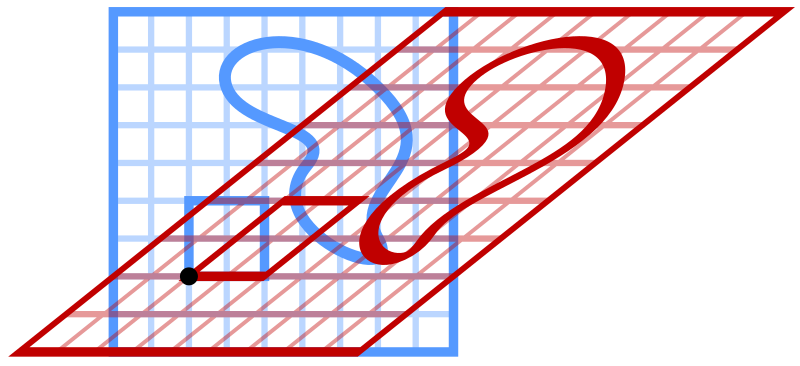
\includegraphics[width=6in]{images/front.png}\\
\vspace{30pt}
\Huge
אלגברה ב' (104168)
\\
אביב 2025
\\
רשימות תרגולים
\vspace{30pt}
\\
\huge
אלן סורני
\vspace{30pt}
\\
\Large
הרשימות עודכנו לאחרונה בתאריך ה־%
\today
}
\date{}

\begin{document}
\frontmatter
\maketitle
\tableofcontents

\mainmatter

\section*{סימונים}

\begin{itemize}
\item[-]
$\brs{n} = \set{1, \ldots, n}$.
\item[-]
$\sum_{i \in \brs{n}} a_i = \sum_{i=1}^n a_i = a_1 + a_2 + \ldots + a_n$
\item[-] $\Mat_{m \times n}\prs{\mbb{F}}$ הוא מרחב המטריצות עם
$m$
שורות ו־%
$n$
עמודות, עם מקדמים בשדה
$\mbb{F}$.
\item[-]
$\mbb{F}^n = \Mat_{n \times 1}\prs{\mbb{F}}$
\item[-]
$\Mat_{n}\prs{\mbb{F}} = \Mat_{n \times n}\prs{\mbb{F}}$
\item[-]
$\hom_{\mbb{F}}\prs{V,W}$
הוא מרחב ההעתקות הלינאריות
$V \to W$
כאשר
$V,W$
מרחבים וקטוריים מעל
$\mbb{F}$.
\item[-]
$\End_{\mbb{F}}\prs{V} = \hom_{\mbb{F}}\prs{V,V}$
\end{itemize}

\part{חלק ראשון - מרחבים שמורים}

\chapter{חזרה על מטריצות מייצגות}

\section{הגדרות ותכונות בסיסיות}

\begin{definition}[וקטור קואורדינטות]
יהי
$V$
מרחב וקטורי סוף־מימדי מעל שדה
$\mbb{F}$,
יהי
$B = \prs{v_1, \ldots, v_n}$
בסיס של
$V$
ויהי
$v \in V$.
\emph{וקטור הקואורדינטות של
$v$
לפי הבסיס
$B$}
הוא הוקטור
$\brs{v}_B = \pmat{\alpha_1 \\ \vdots \\ \alpha_n}$
כאשר
$\alpha_1, \ldots, \alpha_n \in \mbb{F}$
היחידים עבורם
\[\text{.}v = \sum_{i \in [n]} \alpha_i v_i \coloneqq \alpha_1 v_1 + \ldots + \alpha_n v_n\]
\end{definition}

\begin{remark}
ההעתקה
\begin{align*}
\rho_B \colon V &\to \mbb{F}^n \\
v &\mapsto \brs{v}_B
\end{align*}
היא איזומורפיזם לינארי.
\end{remark}

\begin{definition}[מטריצה מייצגת]
יהיו
$V,W$
מרחבים וקטורים סוף־מימדיים מעל אותו שדה
$\mbb{F}$
עם בסיסים
$B,C$
בהתאמה, ונסמן
\[\text{.} B = \prs{v_1, \ldots, v_n}\]
נסמן גם
$n \coloneqq \dim\prs{V}$
ו־%
$m \coloneqq \dim\prs{W}$.
עבור
$T \in \Hom_{\mbb{F}}\prs{V,W}$
נגדיר
\[\text{.} \brs{T}^B_C = \pmat{\vert & & \vert \\ \brs{T\prs{v_1}}_C & \cdots & \brs{T\prs{v_n}}_C \\ \vert & & \vert} \in \Mat_{m \times n}\prs{\mbb{F}}\]
\end{definition}

\begin{theorem}[כפל מטריצות]
תהי
$A \in \Mat_{m \times n}\prs{\mbb{F}}$
ויהי
$E = \prs{e_1, \ldots, e_m}$
הבסיס הסטנדרטי של
$\mbb{F}^n$.
אז:
\begin{enumerate}[label = (\roman*)]
\item
לכל
$i \in [m]$
מתקיים כי
$A e_i$
העמודה ה־%
$i$
של
$A$.
\item
לכל
$B = \pmat{\vert & & \vert \\ b_1 & \cdots & b_\ell \\ \vert & & \vert} \in \Mat_{n \times \ell}\prs{\mbb{F}}$
מתקיים
$AB = \pmat{\vert & & \vert \\ A b_1 & \cdots & A b_\ell \\ \vert & & \vert}$.
\end{enumerate}
\end{theorem}

\begin{exercisechap}
הראו שניתן לשחזר את ההגדרה של כפל מטריצות משתי התכונות במשפט.
\end{exercisechap}

\begin{remark}
ההעתקה
\begin{align*}
\eta^B_C \colon \Hom_{\mbb{F}}\prs{V,B} &\to \Mat_{m \times n}\prs{\mbb{F}} \\
T &\mapsto \brs{T}^B_C
\end{align*}
היא איזומורפיזם לינארי.
\end{remark}

\begin{proposition}
תהי
$T \in \Hom_{\mbb{F}}\prs{V,W}$
ויהיו
$B = \prs{v_1, \ldots, v_n}$
בסיס של
$V$
ו־%
$C$
בסיס של
$W$.
אז
\[\brs{T}^B_C \brs{v}_B = \brs{T\prs{v}}_C\]
לכל
$v \in V$.
\end{proposition}

\begin{notation}
אם
$B$
בסיס של מרחב וקטורי סוף־מימדי
$V$
ואם
$T \in \End\prs{V}$,
נסמן
$\brs{T}_B \coloneqq \brs{T}^B_B$
ונקרא למטריצה זאת
\emph{המטריצה המייצגת של
$T$
לפי הבסיס
$B$}.
\end{notation}

\begin{notation}
יהי
$V$
מרחב וקטורי סוף־מימדי עם בסיסים
$B,C$.
נסמן
$M^B_C \coloneqq \brs{\id_V}^B_C$.
\end{notation}

\begin{notation}
אם
$A \in \Mat_{n\times n}\prs{\mbb{F}}$,
נסמן
\begin{align*}
T_A \colon \mbb{F}^n &\to \mbb{F}^n \\
\text{.} \hphantom{lalala} v &\mapsto Av
\end{align*}
\end{notation}

\section{תרגילים}

\begin{exercisechap}\label{ex:p(x+1)}
יהי
$V = \mbb{R}_3\brs{x}$
מרחב הפולינום הממשיים ממעלה לכל היותר
$3$,
תהי
\begin{align*}
T \colon \mbb{R}_3\brs{x} &\to \mbb{R}_3\brs{x} \\
p\prs{x} &\mapsto p\prs{x+1}
\end{align*}
ויהי
$B = \prs{1,x,x^2,x^3}$
בסיס של
$V$.
כיתבו את
$\brs{T}_B$.
\end{exercisechap}

\begin{solution}
לפי הגדרת המטריצה המייצגת,
עמודות
$\brs{T}_B$
הן
$\brs{T\prs{x^i}}_B$
עבור
$i \in \set{0,1,2,3}$.
מתקיים
\begin{align*}
T\prs{1} &= 1 \\
T\prs{x} &= x+1 = 1 + x \\
T\prs{x^2} &= \prs{x+1}^2 = 1 + 2x + x^2 \\
T\prs{x^3} &= \prs{x+1}^3 = 1 + 3x + 3x^2 + x^3
\end{align*}
ולכן
\begin{align*}
\brs{T\prs{1}}_B &= e_1 \\
\brs{T\prs{x}}_B &= e_1 + e_2 \\
\brs{T\prs{x^2}}_B &= e_1 + 2 e_2 + e_3 \\
\brs{T\prs{x^3}}_B &= e_1 + 3 e_2 + 3 e_3 + e_4
\end{align*}
ואז
\begin{align*}
\text{.} \brs{T}_B &= \pmat{1 & 1 & 1 & 1 \\ 0 & 1 & 2 & 3 \\ 0 & 0 & 1 & 3 \\ 0 & 0 & 0 & 1}
\end{align*}
\end{solution}

\begin{exercisechap}
יהי
$V = \Mat_{2 \times 2}\prs{\mbb{C}}$,
תהי
\begin{align*}
T \colon V &\to V \\
A &\mapsto \frac{1}{2} \prs{A - A^t}
\end{align*}
ויהי
\[E = \prs{E_{1,1}, E_{1,2}, E_{2,1}, E_{2,2}} \coloneqq \pmat{\pmat{1 & 0 \\ 0 & 0}, \pmat{0 & 1 \\ 0 & 0}, \pmat{0 & 0 \\ 1 & 0}, \pmat{0 & 0 \\ 0 & 1}}\]
\emph{הבסיס הסטנדרטי של
$V$}.
כיתבו את
$\brs{T}_E$.
\end{exercisechap}

\begin{solution}
כמו מקודם, נחשב את
$\brs{T\prs{E_{i,j}}}_E$
כיוון שאלו עמודות
$\brs{T}_E$.
מתקיים
\begin{align*}
T\prs{E_{1,1}} &= \frac{1}{2} \prs{E_{1,1} - E_{1,1}} = 0 \\
T\prs{E_{1,2}} &= \frac{1}{2} \prs{\pmat{0 & 1 \\ 0 & 0} - \pmat{0 & 0 \\ 1 & 0}} = \frac{1}{2} E_{1,2} - \frac{1}{2} E_{2,1} \\
T\prs{E_{2,1}} &= \frac{1}{2} \prs{E_{2,1} - E_{1,2}} = \frac{1}{2} E_{2,1} - \frac{1}{2} E_{1,2} \\
\text{,} T\prs{E_{2,2}} &= \frac{1}{2} \prs{E_{2,2} - E_{2,2}} = 0 \\
\end{align*}
לכן
\begin{align*}
\brs{T\prs{E_{1,1}}}_E &= 0 \\
\brs{T\prs{E_{1,2}}}_E &= \frac{1}{2} e_2 - \frac{1}{2} e_3 \\
\brs{T\prs{E_{2,1}}}_E &= -\frac{1}{2} e_2 + \frac{1}{2} e_3 \\
\brs{T\prs{E_{2,2}}}_E &= 0
\end{align*}
ואז
\begin{align*}
\text{,} \brs{T}_E &= \pmat{0 & 0 & 0 & 0 \\ 0 & \frac{1}{2} & -\frac{1}{2} & 0 \\ 0 & -\frac{1}{2} & \frac{1}{2} & 0 \\ 0 & 0 & 0 & 0}
\end{align*}
כנדרש.
\end{solution}

\begin{exercisechap}
יהי
$V = \Hom_{\mbb{R}}\prs{\mbb{R}^2, \mbb{R}}$
עם הבסיס
$B = \prs{f_1, f_2}$
כאשר
\begin{align*}
f_1\prs{\pmat{x \\ y}} &= x \\
\text{,} f_2\prs{\pmat{x \\ y}} &= y
\end{align*}
ותהי
\begin{align*}
\text{.} A &= \pmat{1 & 2 \\ 3 & 4} \in \Mat_{2 \times 2}\prs{\mbb{R}}
\end{align*}
מיצאו
$T \in \End_{\mbb{R}}\prs{V}$
עבורו
$\brs{T}_B = A$.
\end{exercisechap}

\begin{solution}
עבור
$T \in \End_{\mbb{R}}\prs{V}$
מתקיים
\[\text{.} \brs{T}_B = \pmat{\vert & \vert \\ \brs{T\prs{f_1}}_B & \brs{T\prs{f_2}}_B \\ \vert & \vert}\]
לכן נדרוש
\begin{align*}
\brs{T\prs{f_1}}_B &= \pmat{1 \\ 2} \\
\text{.} \brs{T\prs{f_2}}_B &= \pmat{3 \\ 4}
\end{align*}
אז
\begin{align*}
T\prs{f_1} &= f_1 + 2 f_2 \\
\text{.} T\prs{f_2} &= 3 f_1 + 4 f_2
\end{align*}
לכן, אם
$f \in V$
איבר כללי, נכתוב
\[f\pmat{x\\y} = \alpha x + \beta y = \alpha f_1 \pmat{x \\ y} + \beta f_2\pmat{x \\ y}\]
ונקבל כי
\begin{align*}
\prs{T\prs{f}}\pmat{x\\y} &= \prs{T\prs{\alpha f_1 + \beta f_2}}\pmat{x\\y}
\\&= \alpha T\prs{f_1}\pmat{x\\y} + \beta T\prs{f_2} \pmat{x\\y}
\\&= \alpha \prs{f_1 + 2 f_2}\pmat{x\\y} + \beta \prs{3 f_1 + 4 f_2} \pmat{x\\y}
\\ \text{.} \hphantom{\prs{T\prs{f}}\pmat{x\\y}} &= \alpha \prs{x + 2 y} + \beta \prs{3 x + 4y}
\end{align*}
\end{solution}

\begin{exercisechap}
תהיינה
$A,B \in \Mat_{m \times n}\prs{\mbb{F}}$
ונניח כי לכל
$v \in \mbb{F}^n$
מתקיים
$Av = Bv$.
אז
$A = B$.
\end{exercisechap}

\begin{solution}
מהנתון, מתקיים
$\prs{A - B}v = 0$
לכל
$v \in \mbb{F}^n$.
בפרט העמודה ה־%
$i$
של
$A-B$,
שהינה
$\prs{A - B}e_i$,
שווה ל־%
$0$.
לכן
$A - B = 0$.
\end{solution}

\begin{proposition}
יהיו
$U,V,W$
מרחבים וקטוריים סוף־מימדיים מעל אותו שדה
$\mbb{F}$
עם בסיסים
$B,C,D$
בהתאמה,
ותהיינה
\begin{align*}
S \in \Hom_{\mbb{F}}\prs{U,V} \\
\text{.} T \in \Hom_{\mbb{F}}\prs{V,W}
\end{align*}
אז
\[\text{.} \brs{T \circ S}^B_D = \brs{T}^C_D \brs{S}^B_C\]
\end{proposition}

\begin{exercisechap} \label{exercisechap:change-of-basis-through-isomorphism}
יהיו
$V,W$
מרחבים וקטוריים סוף־מימדיים מעל שדה
$\mbb{F}$
ותהי
$T \in \Hom_{\mbb{F}}\prs{V,W}$
חד־חד ערכית.

יהיו
\begin{align*}
B &= \prs{v_1, \ldots, v_n} \\
C &= \prs{u_1, \ldots, u_n}
\end{align*}
בסיסים של
$V$
ויהיו
\begin{align*}
B' &= \prs{T\prs{v_1}, \ldots, T\prs{v_n}} \\
\text{.} C' &= \prs{T\prs{u_1}, \ldots, T\prs{u_n}}
\end{align*}
אז
$B',C'$
בסיסים של
$\im\prs{T} = \set{T\prs{v}}{v \in V}$
וגם
$M^B_C = M^{B'}_{C'}$.
\end{exercisechap}

\begin{solution}
כיוון ש־%
$T$
חד־חד ערכית ועל התמונה, צמצום הטווח נותן איזומורפיזם
$T \colon V \riso \im\prs{T}$.
איזומורפיזם שולח בסיס לבסיס, לכן
$B',C'$
בסיסים.

כעת, לכל
$i \in [n]$
נכתוב
\begin{align*}
v_i &= \sum_{j \in \brs{n}} \alpha_{i,j} u_i
\end{align*}
ואז
\begin{align*}
\text{.} M^B_C e_i = \brs{v_i}_C = \pmat{\alpha_{i,1} \\ \vdots \\ \alpha_{i,n}}
\end{align*}
כמו כן,
\begin{align*}
T\prs{v_i}
&=
T\prs{\sum_{i \in [n]} \alpha_{i,j} u_j}
\\&=
\sum_{i \in [n]} \alpha_{i,j} T\prs{u_j}
\end{align*}
ולכן גם
\[\text{.} M^{B'}_{C'} e_i = \brs{T\prs{v_i}}_{C'} = \pmat{\alpha_{i,1} \\ \vdots \\ \alpha_{i,n}}\]
קיבלנו כי כל עמודות המטריצות שוות, ולכן יש שוויון.
\end{solution}

\begin{exercisechap}
תהי
$A \in \Mat_{n \times n}\prs{\mbb{F}}$
הפיכה.
\begin{enumerate}
\item יהי
$E$
הבסיס הסטנדרטי של
$\mbb{F}^n$.
מיצאו בסיס
$B$
של
$\mbb{F}^n$
עבורו
$A = M^B_E$.

\item
מיצאו בסיס
$C$
של
$\mbb{F}^n$
עבורו
$A = M^E_C$.

\item \emph{
(לא הספקנו בתרגול)
}
יהי
$B$
בסיס של
$\mbb{F}^n$.
מיצאו בסיס
$C$
של
$\mbb{F}^n$
עבורו
$A = M^B_C$.

\item \emph{
(לא הספקנו בתרגול)
}
יהי
$V$
מרחב וקטורי ממימד
$n \in \mbb{N}_+$
מעל
$\mbb{F}$,
יהי
$T \in \End_{\mbb{F}}\prs{V}$
איזומורפיזם
ויהי
$B = \prs{v_1, \ldots, v_n}$
בסיס של
$V$.
מיצאו בסיס
$C$
של
$V$
עבורו
$\brs{T}^B_C = A$.
\end{enumerate}
\end{exercisechap}

\begin{solution}
\begin{enumerate}
\item
אם
$B = \prs{v_1, \ldots, v_n}$,
מתקיים מההגדרה כי
\[\text{.} M^B_E = \pmat{\vert & & \vert \\ \brs{v_1}_E & \cdots & \brs{v_n}_E \\ \vert & & \vert} = \pmat{\vert & & \vert \\ v_1 & \cdots & v_n \\ \vert & & \vert}\]
לכן ניקח את
$\prs{v_1, \ldots, v_n}$
להיות עמודות
$A$,
לפי הסדר.

\item
לכל
$v \in \mbb{F}^n$
מתקיים
\[M^C_E M^E_C v = M^C_E \brs{v}_C = \brs{v}_E = v\]
ולכן
$M^E_C = \prs{M^C_E}^{-1}$.
אם ניקח
$C = \prs{u_1, \ldots, u_n}$
כאשר
$u_i$
העמודה ה־%
$i$
של
$A^{-1}$
נקבל מהסעיף הקודם כי
$M^C_E = A^{-1}$
ולכן
$M^E_C = \prs{A^{-1}}^{-1} = A$.
כלומר ניקח,
$u_i = A^{-1} e_i$.

\item
מתקיים
$M^B_C = M^E_C M^B_E$
לכן נרצה שיתקיים
$M^E_C M^B_E = A$
או במילים אחרות
$M^E_C = A \prs{M^B_E}^{-1} = A M^E_B$.
מהסעיף הקודם, נרצה
$C = \prs{u_1, \ldots, u_n}$
כאשר
$u_i$
העמודה ה־%
$i$
של
$\prs{A M^E_B}^{-1} = M^B_E A^{-1}$,
כלומר
\[\text{.} u_i = M^B_E A^{-1} e_i\]

\item
עבור כל בסיס
$C'$
מתקיים
$\brs{T}^B_{C'} = M^B_{C'} \brs{T}^B_B$
לכן נרצה
$M^B_C \brs{T}^B_B = A$.
כיוון ש־%
$T$
איזומורפיזם, המטריצה
$\brs{T}^B_B$
הפיכה, ולכן נרצה
$M^B_C = A \prs{\brs{T}^B_B}^{-1}$.
כעת, אם
$C = \prs{v_1, \ldots, v_n}$
נקבל לפי
\ref{proposition:change-of-basis-through-isomorphism}
עבור האיזומורפיזם
$\rho_B$
כי
$M^B_C = M^E_{\hat{C}}$
כאשר
$\hat{C} = \prs{\brs{v_1}_B, \ldots, \brs{v_n}_B}$.
לכן נחפש
$\hat{C}$
עבורו
$M^E_{\hat{C}} = A \brs{T}_B^{-1}$.
לפי הסעיף השני, נרצה
$\hat{C} = \prs{u_1, \ldots, u_n}$
עבור
\[\text{.} u_i = \prs{A \brs{T}_B^{-1}}^{-1} e_i = \brs{T}_B A^{-1} e_i\]
לכן
\[\text{.} v_i = \rho_B^{-1} \prs{\brs{T}_B A^{-1} e_i}\]
\end{enumerate}
\end{solution}

\begin{exercisechap}[לא הספקנו בתרגול]
יהי
$V = \mbb{C}_3\brs{x}$,
תהי
\begin{align*}
T \colon V &\to V \\
\text{,} \hphantom{lalala} p\prs{x} &\mapsto p\prs{x+1}
\end{align*}
יהי
$E = \pmat{1,x,x^2,x^3}$,
\emph{הבסיס הסטנדרטי}
ותהי
$A = \pmat{0 & 1 & 0 & 0 \\ 1 & 0 & 0 & 0 \\ 0 & 0 & 0 & 1 \\ 0 & 0 & 1 & 0}$.
כיתבו מפורשות בסיס
$C$
של
$V$
עבורו
$A = \brs{T}^E_C$.
\end{exercisechap}

\begin{solution}
לפי התרגיל הקודם, נרצה קודם
$\hat{C} = \prs{u_1, \ldots, u_4}$
כאשר
$u_i = \brs{T}_E A^{-1} e_i$.
חישבנו ב־%
\ref{ex:p(x+1)}
כי
\[\brs{T}_E = \pmat{1 & 1 & 1 & 1 \\ 0 & 1 & 2 & 3 \\ 0 & 0 & 1 & 3 \\ 0 & 0 & 0 & 1}\]
וניתן לראות כי
$A^2 = I$
כלומר
$A^{-1} = A$.
נשים לב כי
\begin{align*}
A e_1 &= e_2 \\
A e_2 &= e_1 \\
A e_3 &= e_4 \\
A e_4 &= e_3
\end{align*}
ואז נקבל
\begin{align*}
u_1 &= \brs{T}_E A^{-1} e_1 = \brs{T}_E e_2 = \pmat{1 \\ 1 \\ 0 \\ 0} \\
u_2 &= \brs{T}_E A^{-1} e_2 = \brs{T}_E e_1 = \pmat{1 \\ 0 \\ 0 \\ 0} \\
u_3 &= \brs{T}_E A^{-1} e_3 = \brs{T}_E e_4 = \pmat{1 \\ 3 \\ 3 \\ 1} \\
\text{,} u_4 &= \brs{T}_E A^{-1} e_4 = \brs{T}_E e_3 = \pmat{1 \\ 2 \\ 1 \\ 0}
\end{align*}
כלומר
\[\text{,} \hat{C} = \prs{\pmat{1 \\ 1 \\ 0 \\ 0}, \pmat{1 \\ 0 \\ 0 \\ 0}, \pmat{1 \\ 3 \\ 3 \\ 1}, \pmat{1 \\ 2 \\ 1 \\ 0}}\]
ולבסוף
\[\text{.} C = \prs{v_1, v_2, v_3, v_4} \coloneqq \prs{1+x, 1, 1+3x+3x^2+x^3, 1+2x+x^2}\]

ליתר ביטחון, נבדוק שהמטריצה המייצגת היא אכן
$A$.
מתקיים
\begin{align*}
T\prs{1} &= 1 = v_2 \\
T\prs{x} &= x+1 = v_1 \\
T\prs{x^2} &= \prs{x+1}^2 = 1+2x+x^2 = v_4 \\
T\prs{x^3} &= \prs{x+1}^3 = 1+3x+3x^2+x^3 = v_3
\end{align*}
ולכן
\begin{align*}
\brs{T}^E_C &= \pmat{\vert & \vert & \vert & \vert \\ \brs{T\prs{1}}_C & \brs{T\prs{x}}_C & \brs{T\prs{x^2}}_C & \brs{T\prs{x^3}}_C \\ \vert & \vert & \vert & \vert}
\\&= \pmat{\vert & \vert & \vert & \vert \\ \brs{v_2}_C & \brs{v_1}_C & \brs{v_4}_C & \brs{v_3}_C \\ \vert & \vert & \vert & \vert}
\\&= \pmat{\vert & \vert & \vert & \vert \\ e_2 & e_1 & e_4 & e_3 \\ \vert & \vert & \vert & \vert}
\\&= A
\end{align*}
כנדרש.
\end{solution}

\chapter{הדטרמיננטה}

\section{הגדרות ותכונות בסיסיות}

\begin{definition}[דטרמיננטה]
תהי
$A \in \Mat_{n \times n}\prs{\mbb{F}}$
מטריצה עם מקדמים בשדה
$\mbb{F}$.
נגדיר את
\emph{הדטרמיננטה}
$\det\prs{A}$
של
$A$
באופן הרקורסיבי הבא.

תהי
$A_{\prs{i,j}}$
המטריצה המתקבלת מ־%
$A$
על ידי הסרת השורה ה־%
$i$
והעמודה ה־%
$j$.
המספר
$\det\pr{A_{\pr{i,j}}}$
נקרא
\emph{המינור}
ה־$\prs{i,j}$ של
$A$
והדטרמיננטה של
$A$
שווה
\begin{align*}
\det\prs{A} &= \sum_{i \in \brs{n}} \prs{-1}^{i+j} a_{i,j} \det\prs{A_{\prs{i,j}}}
\end{align*}
עבור כל
$j \in \brs{n}$
קבוע, ושווה
\begin{align*}
\det\prs{A} &= \sum_{j \in \brs{n}} \prs{-1}^{i+j} a_{i,j} \det\prs{A_{\prs{i,j}}}
\end{align*}
עבור כל
$i \in \brs{n}$
קבוע.
\end{definition}

\begin{theorem}
תהיינה
$A, B, C \in \Mat_{n \times n}\prs{\mbb{F}}$
ונניח כי
$C$
הפיכה.
מתקיימות התכונות הבאות.
\begin{enumerate}
\item $\det\prs{AB} = \det\prs{A} \cdot \det\prs{B}$
\item $\det\prs{C^{-1}} = \prs{\det\prs{C}}^{-1}$
\end{enumerate}
\end{theorem}

\begin{theorem}
\begin{enumerate}
\item החלפת שתי שורות או עמודות במטריצה כופלת את הדטרמיננטה ב־%
$\prs{-1}$.
\item כפל שורה או עמודה במטריצה בסקלר
$\alpha$
כופל את הדטרמיננטה ב־%
$\alpha$.
\item הוספת כפולה שורה או עמודה לשורה או עמודה במטריצה אינה משנה את הדטרמיננטה.
\end{enumerate}
\end{theorem}

\section{תרגילים}

\begin{exercisechap}
חשבו את הדטרמיננטות של המטריצות הבאות.

\begin{enumerate}
\item \[\pmat{1 & 2 & 3 \\ 4 & 5 & 6 \\ 7 & 8 & 9} \in \Mat_{3}\prs{\mbb{R}}\]
\item \[\pmat{0 & 0 & 0 & 1 \\ 0 & 0 & 1 & 0 \\ 0 & 1 & 0 & 0 \\ 1 & 0 & 0 & 0} \in \Mat_{4}\prs{\mbb{R}}\]
\item \[\pmat{1 & 0 & 0 \\ 0 & 1 & 0 \\ 1 & 1 & 1} \in \Mat_{3}\prs{\mbb{R}}\]
\item \[\pmat{1 & 0 & 1 \\ 0 & 1 & 0 \\ 1 & 1 & 1} \in \Mat_{3}\prs{\mbb{R}}\]
\end{enumerate}
\end{exercisechap}

\begin{solution}
\begin{enumerate}
\item
נחשב לפי השורה הראשונה.
\begin{align*}
\det \pmat{1 & 2 & 3 \\ 4 & 5 & 6 \\ 7 & 8 & 9} &= 1 \cdot \det\pmat{5 & 6 \\ 8 & 9} - 2 \cdot \det \pmat{4 & 6 \\ 7 & 9} + 3 \cdot \det \pmat{4 & 5 \\ 7 & 8}
\\&=
1 \cdot \prs{5 \cdot 9 - 6 \cdot 8} - 2 \cdot \prs{4 \cdot 9 - 6 \cdot 7} + 3 \cdot \prs{4 \cdot 8 - 5 \cdot 7}
\\&=
1 \cdot \prs{-3} -2 \cdot \prs{-6} + 3 \cdot \prs{-3}
\\&=
-3 + 12 - 9
\\&= 0
\end{align*}
\item החלפת שורות כופלת את הדטרמיננטה ב־%
$\prs{-1}$.
כיוון שניתן לקבל את המטריצה ממטריצת היחידה על ידי החלפת השורות
$1,4$
והשורות
$2,3$,
נקבל כי הדטרמיננטה שווה לזאת של היחידה. לכן
\[\text{.} \det \pmat{0 & 0 & 0 & 1 \\ 0 & 0 & 1 & 0 \\ 0 & 1 & 0 & 0 \\ 1 & 0 & 0 & 0} = 1\]
\item
הוספת כפולה של השורות הראשונה והשנייה ב־%
$\prs{-1}$
לשורה השלישית לא משנה את הדרמיננטה. לכן הדטמיננטה של המטריצה שווה לזאת של היחידה, ולכן
\[\text{.} \det \pmat{1 & 0 & 0 \\ 0 & 1 & 0 \\ 1 & 1 & 1} = 1\]
\item
הוספת כפולה של השורות הראשונה והשנייה ב־%
$\prs{-1}$
לשורה השלישית לא משנה את הדרמיננטה. לכן הדטמיננטה של המטריצה שווה לזאת של
\begin{align*}
\text{.} \pmat{1 & 0 & 1 \\ 0 & 1 & 0 \\ 0 & 0 & 0}
\end{align*}
כיוון שהשורה השלישית היא שורת אפסים, אם נפתח את הדטרמיננטה לפיה נקבל שהדטרמיננטה שווה
$0$.
זה נכון באופן כללי יותר אם השורות תלויות לינארית, כי נוכל לקבל שורת אפסים מצירוף לינארי של השורות.
\end{enumerate}
\end{solution}

\begin{exercisechap}
תהי
$T \in \End_{\mbb{F}}\prs{V}$
העתקה לינארית ויהי
$B$
בסיס של
$V$.
הראו כי ניתן להגדיר
$\det\prs{T} = \det\prs{\brs{T}_B}$.
כלומר, הראו שאם
$C$
בסיס נוסף של
$V$
מתקיים
$\det\prs{\brs{T}_B} = \det\prs{\brs{T}_C}$.
\end{exercisechap}

\begin{solution}
מתקיים
\begin{align*}
\brs{T}_B = \prs{M^B_C}^{-1} \brs{T}_C M^B_C
\end{align*}
ולכן
\begin{align*}
\text{.} \det\prs{\brs{T}_B} &= \det\prs{\prs{M^B_C}^{-1}} \det\prs{\brs{T}_C} \det\prs{M^B_C}
\end{align*}
כיוון ש־%
$\det\prs{A^{-1}} = \frac{1}{\det\prs{A}}$
 לכל מטריצה
 $A$,
 מתקיים
 $\det\prs{\prs{M^B_C}^{-1}} = \frac{1}{\det\prs{M^B_C}}$.
 לכן, נקבל בסה"כ כי
 \[\text{,} \det\prs{\brs{T}_B} = \det\prs{\brs{T}_C}\]
 כנדרש.
\end{solution}

\chapter{המטריצה המצורפת וכלל קרמר}

\section{הגדרות ותכונות בסיסיות}

\begin{definition}[המטריצה המצורפת]
תהי
$A \in \Mat_{n}\prs{\mbb{F}}$.
\emph{המטריצה המצורפת של
$A$}
היא המטריצה
$\adj\prs{A} \in \Mat_n\prs{\mbb{F}}$
המקיימת
\begin{align*}
\text{.} \adj\prs{A}_{i,j} = \prs{-1}^{i+j} \det\prs{A_{\prs{j,i}}}
\end{align*}
\end{definition}

\begin{proposition}
עבור
$A \in\Mat_n\prs{\mbb{F}}$
מתקיים
\begin{align*}
\text{.} A \adj\pr{A} = \adj\prs{A} A = \det\prs{A} I_n
\end{align*}
\end{proposition}

\begin{corollary}
עבור
$A \in \Mat_n\prs{\mbb{F}}$
הפיכה מתקיים
\begin{align*}
\text{.} A^{-1} = \frac{1}{\det\prs{A}} \adj\prs{A}
\end{align*}
\end{corollary}

\begin{theorem}[כלל קרמר]
תהי
$A \in \Mat_n\prs{\mbb{F}}$
הפיכה, ויהי
$b \in \mbb{F}^n$.
עבור כל
$i \in\brs{n}$,
נסמן ב־%
$A_i$
את המטריצה המתקבלת על ידי החלפת העמודה ה־%
$i$
של
$A$
ב־%
$b$.
אז, למשוואה
$Ax = b$
קיים פתרון יחיד
$x \coloneqq \prs{x_i}_{i \in \brs{n}} \in \mbb{F}^n$
הנתון על ידי
\begin{align*}
\text{.} \forall i \in \brs{n} \colon x_i = \frac{\det\prs{A_i}}{\det\prs{A}}
\end{align*}
\end{theorem}

\section{תרגילים}

\begin{exercisechap}
תהי
$A = \pmat{1 & -1 & 2 \\ 2 & 3 & 5 \\ -2 & 0 & 1} \in \Mat_3\prs{\mbb{R}}$.
חשבו את
$\adj\pr{A}$.
\end{exercisechap}

\begin{solution}
נחשב את
$\adj\prs{A}$
לפי ההגדרה.
\begin{align*}
\adj\prs{A} &= \pmat{\det\pmat{3 & 5 \\ 0 & 1} & -\det\pmat{-1 & 2 \\ 0 & 1} & \det\pmat{-1 & 2 \\ 3 & 5} \\
-\det\pmat{2 & 5 \\ -2 & 1} & \det\pmat{1 & 2 \\ -2 & 1} & -\det\pmat{1 & 2 \\ 2 & 5} \\
\det\pmat{2 & 3 \\ -2 & 0} & -\det\pmat{1 & -1 \\ -2 & 0} & \det\pmat{1 & -1 \\ 2 & 3}}
\\&=
\pmat{3 & 1 & -11 \\ -12 & 5 & -1 \\ 6 & 2 & 5}
\end{align*}
\end{solution}

\begin{exercisechap}
היעזרו במטריצה המצורפת כדי לחשב את ההופכית עבור כל אחת מהמטריצות הבאות.

\begin{align*}
A &= \pmat{-2 & 3 & 2 \\ 6 & 0 & 3 \\ 4 & 1 & -1} \in \Mat_3\prs{\mbb{R}} \\
B &= \pmat{\cos{\theta} & 0 & -\sin{\theta} \in \Mat_3\prs{\mbb{R}} \\
0 & 1 & 0 \\
\sin{\theta} & 0 & \cos{\theta}}
\end{align*}
עבור
$\theta \in \mbb{R}$.
\end{exercisechap}

\begin{solution}
עבור כל אחת משתי המטריצות, נחשב את הדטרמיננטה ואת המטריצה המצורפת שלה.
מתקיים
\begin{align*}
\det\prs{A} &= -2 \det\pmat{0 & 3 \\ 1 & -1} - 3 \det\pmat{6 & 3 \\ 4 & -1} + 2 \det\pmat{6 & 0 \\ 4 & 1}
\\&= -2 \cdot \prs{-3} - 3 \cdot \prs{-18} + 2 \cdot 6
\\&= 72 \\
\det\prs{B} &= 0 + 1 \cdot \det\pmat{\cos{\theta} & -\sin{\theta} \\ \sin{\theta} & \cos{\theta}} - 0
\\&= \cos^2{\theta} + \sin^2{\theta}
\\&= 1
\end{align*}
וכן
\begin{align*}
\adj\prs{A} &= \pmat{\det\pmat{0 & 3 \\ 1 & -1} & -\det\pmat{6 & 3 \\ 4 & -1} & \det\pmat{6 & 0 \\ 4 & 1} \\
-\det\pmat{3 & 2 \\ 1 & -1} & \det\pmat{-2 & 2 \\ 4 & -1} & -\det\pmat{-2 & 3 \\ 4 & 1} \\
\det\pmat{3 & 2 \\ 0 & 3} & -\det\pmat{-2 & 2 \\ 6 & 3} & \det\pmat{-2 & 3 \\ 6 & 0}}^t
\\&= \pmat{-3 & 18 & 6 \\ 5 & -6 & 14 \\ 9 & 18 & -18}^t
\\&= \pmat{-3 & 5 & 9 \\ 18 & -6 & 18 \\ 6 & 14 & -18} \\
\adj\prs{B} &= \pmat{
\det\pmat{1 & 0 \\ 0 & \cos\theta} & -\det\pmat{0 & 0 \\ \sin \theta & \cos \theta} & \det\pmat{0 & 1 \\ \sin\theta & 0} \\
-\det\pmat{0 & - \sin\theta \\ 0 & \cos\theta} & \det\pmat{\cos \theta & - \sin \theta \\ \sin\theta & \cos\theta} & -\det\pmat{\cos \theta & 0 \\ \sin \theta & 0} \\
\det\pmat{0 & -\sin\theta \\ 1 & 0} & -\det\pmat{\cos \theta & - \sin \theta \\ 0 & 0} & \det\pmat{\cos\theta & 0 \\ 0 & 1}}^t
\\&=
\pmat{\cos\theta & 0 & -\sin\theta \\ 0 & 1 & 0 \\ \sin \theta & 0 & \cos \theta}^t
\\&=
\pmat{\cos\theta & 0 & \sin\theta \\ 0 & 1 & 0 \\ -\sin \theta & 0 & \cos \theta}
\end{align*}
ולכן נקבל כי
\begin{align*}
A^{-1} &= \frac{1}{\det\prs{A}} \adj\prs{A}
\\&= \frac{1}{72} \pmat{-3 & 5 & 9 \\ 18 & -6 & 18 \\ 6 & 14 & -18}
\\&= \pmat{-1/24 & 5/72 & 1/8 \\ 1/4 & -1/12 & 1/4 \\ 1/12 & 7/36 & -1/4} \\
B^{-1} &= \frac{1}{\det\prs{B}} \adj\prs{B}
\\\text{,} \hphantom{B^{-1}} &= \pmat{\cos\theta & 0 & \sin\theta \\ 0 & 1 & 0 \\ -\sin \theta & 0 & \cos \theta}
\end{align*}
כנדרש.
\end{solution}

\begin{exercisechap}
תהי
$A \in \Mat_n\prs{\mbb{F}}$.
הראו כי
$\adj\prs{\adj\prs{A}} = \det\prs{A}^{n-2} A$.
\end{exercisechap}

\begin{solution}
נניח תחילה כי
$A$
הפיכה.
אז
$\adj\prs{A} = \det\prs{A} A^{-1}$
גם היא הפיכה. לפי אותה נוסחה נקבל כי
\begin{align*}
\adj\prs{\adj\prs{A}} &= \det\prs{\adj\prs{A}} \adj\prs{A}^{-1} \\
\\&= \frac{\det\prs{\adj\prs{A}}}{\det\prs{A}} A
\end{align*}
ולכן נותר להראות כי
\begin{align*}
\text{.} \det\prs{\adj\prs{A}} = \det\prs{A}^{n-1}
\end{align*}
אכן
\begin{align*}
\det\prs{\adj\prs{A}} &= \det\prs{\det\prs{A} A^{-1}}
\\&= \det\prs{A}^n \det\prs{A^{-1}}
\\\text{,}\hphantom{\det\prs{\adj\prs{A}}}&= \det\prs{A}^{n-1}
\end{align*}
כנדרש.

\end{solution}

\begin{exercisechap}
תהי
$A \in \Mat_n\prs{\mbb{F}}$.
הוכיחו את התכונות הבאות.

\begin{enumerate}
\item
$\adj\prs{A^t} = \adj\prs{A}^t$.

\item 
$A$
הפיכה אם ורק אם
$\adj\prs{A}$
הפיכה.

\item
אם
$A$
הפיכה, מתקיים
$\adj\prs{A^{-1}} = \prs{\adj\prs{A}}^{-1}$.
\end{enumerate}
\end{exercisechap}

\begin{solution}
\begin{enumerate}
\item 
לכל
$i,j \in \brs{n}$
מתקיים
\begin{align*}
\text{.} \adj\prs{A^t}_{i,j} = \prs{-1}^{i+j} \det\prs{A^t_{\prs{j,i}}}
\end{align*}
אבל
$A^t_{\prs{j,i}} = \prs{A_{\prs{i,j}}}^t$
ולכן
\begin{align*}
\text{.} \adj\prs{A^t}_{i,j} = \prs{-1}^{i+j} \det\prs{A_{\prs{i,j}}}
\end{align*}
מצד שני,
\begin{align*}
\text{,} \adj\prs{A}^t_{i,j} = \adj\prs{A}_{j,i} = \prs{-1}^{i+j} \det\prs{A_{\prs{i,j}}}
\end{align*}
ולכן מתקיים שוויון
\begin{align*}
\text{,} \adj\prs{A^t} = \adj\prs{A}^t
\end{align*}
כנדרש.

\item
אם
$A$
הפיכה, מתקיים
$\adj\prs{A} = \det\prs{A} A^{-1}$
ולכן גם
$\adj\prs{A}$
הפיכה.

להיפך, אם
$\adj\prs{A}$
הפיכה, גם
$\adj\prs{\adj\prs{A}}$
הפיכה. אך כיוון שמתקיים
$\adj\prs{\adj\prs{A}} = \det\prs{A}^{n-2} A$,
בהכרח גם
$A$
הפיכה (שכן אחרת אגף ימין אינו מטריצה הפיכה).

\item
נניח כי
$A$
הפיכה.
אז
\begin{align*}
\adj\prs{A^{-1}} &= \det\prs{A^{-1}} \prs{A^{-1}}^{-1}
\\&= \frac{1}{\det\prs{A}} A
\end{align*}
וגם
\begin{align*}
\adj\prs{A}^{-1} &= \prs{\det\prs{A} A^{-1}}^{-1}
\\&= \frac{1}{\det\prs{A}} \prs{A^{-1}}^{-1}
\\ \text{.} \hphantom{\adj\prs{A}^{-1}} &= \frac{1}{\det\prs{A}} A
\end{align*}
מכן נסיק כי
\[\text{,} \adj\prs{A^{-1}} = \adj\prs{A}^{-1}\]
כנדרש.
\end{enumerate}
\end{solution}

\begin{exercisechap}
היעזרו בכלל קרמר כדי לפתור את כל אחת ממערכות המשוואות הלינאריות הבאות, מעל
$\mbb{Q}$.

\begin{enumerate}
\item
\begin{align*}
x + y + z &= 11 \\
2x - 6y - z &= 0 \\
3x + 4y + 2z &= 0
\end{align*}
\item
\begin{align*}
3x - 2y &= 7 \\
3y - 2z &= 6 \\
3z - 2x &= -1
\end{align*}
\end{enumerate}
\end{exercisechap}

\begin{solution}
\begin{enumerate}
\item
נכתוב את מערכת המשוואות בעזרת מטריצות, בתור
$A\vec{x} = b$
כאשר
\begin{align*}
\text{.} A = \pmat{1 & 1 & 1 \\ 2 & -6 & -1 \\ 3 & 4 & 2}, \quad
\vec{x} = \pmat{x \\ y \\ z}, \quad
b = \pmat{11 \\ 0 \\ 0}
\end{align*}
מתקיים כי
\begin{align*}
\det\prs{A} &= \det\pmat{-6 & -1 \\ 4 & 2} - \det \pmat{2 & -1 \\ 3 & 2} + \det\pmat{2 & -6 \\ 3 & 4}
\\&= -8 -7 + 26
\\&= 11
\\
\det\prs{A_1} &= 11 \det\pmat{-6 & -1 \\ 4 & 2}
\\&= -88
\\
\det\prs{A_2} &= -11 \det \pmat{2 & -1 \\ 3 & 2}
\\&=
-77
\\
\det\prs{A_3} &= 11 \det\pmat{2 & -6 \\ 3 & 4}
\\&= 11 \cdot 26
\end{align*}
ולכן לפי כלל קרמר
\begin{align*}
x &= \det\prs{A_1} / \det\prs{A} = -8 \\
y &= \det\prs{A_2} / \det\prs{A} = -7 \\
\text{.} z &= \det\prs{A_3} / \det\prs{A} = 26
\end{align*}

\item
נכתוב את מערכת המשוואות בעזרת מטריצות, בתור
$A\vec{x} = b$
כאשר
\begin{align*}
\text{.} A = \pmat{3 & -2 & 0 \\ 0 & 3 & -2 \\ -2 & 0 & 3}, \quad
\vec{x} = \pmat{x \\ y \\ z}, \quad
b = \pmat{7 \\ 6 \\ -1}
\end{align*}
מתקיים כי
\begin{align*}
\det\prs{A} &= 3 \cdot \det\pmat{3 & -2 \\ 0 & 3} + 2 \cdot \det \pmat{0 & -2 \\ -2 & 3}
\\&= 27 - 8
\\&= 19
\\
\det\prs{A_1} &= \det\pmat{7 & -2 & 0 \\ 6 & 3 & -2 \\ -1 & 0 & 3}
\\&= 7 \cdot \det \pmat{3 & -2 \\ 0 & 3} + 2 \cdot \det\pmat{6 & -2 \\ -1 & 3}
\\&= 7 \cdot 9 + 2 \cdot 16
\\&= 63 + 32
\\&= 95
\\
\det\prs{A_2} &= \det\pmat{3 & 7 & 0 \\ 0 & 6 & -2 \\ -2 & -1 & 3}
\\&= 3 \cdot \det\pmat{6 & -2 \\ -1 & 3} - 7 \cdot \det\pmat{0 & -2 \\ -2 & 3}
\\&= 3 \cdot 16 - 7 \cdot \prs{-4}
\\&= 76
\\
\det\prs{A_3} &= \det\pmat{3 & -2 & 7 \\ 0 & 3 & 6 \\ -2 & 0 & -1}
\\&= 3 \cdot \det\pmat{3 & 6 \\ 0 & -1} -2 \cdot \det\pmat{-2 & 7 \\ 3 & 6}
\\&= -9 -2 \cdot \prs{-12 - 21}
\\&= -9 + 66
\\&= 57
\end{align*}
ולכן לפי כלל קרמר
\begin{align*}
x &= \det\prs{A_1} / \det\prs{A} = 95/19 = 5 \\
y &= \det\prs{A_2} / \det\prs{A} = 76/19 = 4 \\
\text{.} z &= \det\prs{A_3} / \det\prs{A} = 57/19 = 3
\end{align*}
\end{enumerate}
\end{solution}

\begin{exercisechap}
תהי
$A \in \Mat_n\prs{\mbb{F}}$,
יהי
$b \in \mbb{F}^n$
ונניח כי
$y \in \mbb{F}^n$
מקיים
$Ay = b$.

תהי
$\tilde{A}$
מטריצה המתקבלת מ־%
$A$
על ידי כפל של העמודה ה־%
$i$
ב־%
$\alpha \in\mbb{R}$.
הראו ישירות לפי כלל קרמר כי
$\tilde{y} = \pmat{y_1 \\ \vdots \\ y_{i-1} \\ y_i/\alpha \\ y_{i+1} \\ y_n}$
פתרון עבור המערכת
$\tilde{A}x = b$.
\end{exercisechap}

\begin{solution}
מתקיים כי
$\det\prs{\tilde{A}} = \alpha \det\prs{A}$.
כמו כן
$\det\prs{\tilde{A}_i} = \det\prs{A_i}$
כיוון שמתקיים
$\tilde{A}_i = A_i$,
ולכל
$j \in \brs{n} \setminus \set{i}$
מתקיים
$\det\prs{\tilde{A}_j} = \alpha \det\prs{A_j}$.

לפי כלל קרמר נקבל כי
$\tilde{y}$
פתרון של המערכת
$\tilde{A} x = b$,
כיוון שמתקיים
\begin{align*}
\det\prs{\tilde{A}_i} / \det\prs{\tilde{A}} &= \det\prs{A_i} / \prs{\alpha \det\prs{A}} = y_i / \alpha
\end{align*}
וכן לכל
$j \in \brs{n} \setminus \set{i}$
מתקיים
\begin{align*}
\text{.} \det\prs{\tilde{A}_j} / \det\prs{\tilde{A}} = \alpha \det\prs{A_j} / \prs{\alpha \det\prs{A}} = \det\prs{A_j} / \det\prs{A} = y_j
\end{align*}
\end{solution}

\printbibliography
\end{document}
